\documentclass[12pt, twoside]{article}
\usepackage[francais]{babel}
\usepackage[T1]{fontenc}
\usepackage[latin1]{inputenc}
\usepackage[left=7mm, right=7mm, top=7mm, bottom=7mm]{geometry}
\usepackage{float}
\usepackage{graphicx}
\usepackage{array}
\usepackage{multirow}
\usepackage{amsmath,amssymb,mathrsfs}
\usepackage{soul}
\usepackage{textcomp}
\usepackage{eurosym}
 \usepackage{variations}
\usepackage{tabvar}


\pagestyle{empty}

\begin{document}


\section*{\center{Devoir maison 4}}


\bigskip





\fbox{

\begin{minipage}{18cm}
\textit{Devoir � rendre sur feuille grand format petits
carreaux pour le \textbf{lundi 8 mars 2010}.}
\end{minipage}
}

\enskip


 \textit{Remarque: La pr�sentation, la pr�cision et la clart� des figures 
 seront pris en compte. }


\enskip


\subsection*{Exercice 1}


Reproduire en vraie grandeur la figure ci-dessous:

\begin{center}
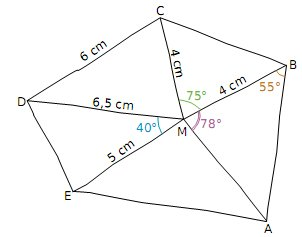
\includegraphics[width=6cm]{images/ex19p122.jpg}
\end{center}





\subsection*{Exercice 2} 

\begin{tabular}{cc}
\begin{minipage}{11cm}
\begin{enumerate}
  \item Calculer la mesure des angles manquants pour les 
  
  triangles DEC, EBC et
  EBA. Justifier votre r�ponse.
  
  
  \item  Les points D, E et A sont-ils align�s? Justifier votre 
 
   r�ponse. 
\end{enumerate}
\end{minipage}
&
\begin{minipage}{7cm}
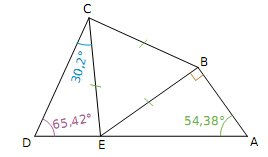
\includegraphics[width=7cm]{images/ex6p120.jpg}
\end{minipage}
\end{tabular}


\textit{Chaque r�sultat sera justifi� par un calcul ou une propri�t� du
  cours.}
  

\subsection*{Exercice 3}

On veut construire un triangle ABC tel que AB=5cm et BC=2cm.

De plus, on veut que la longueur du c�t� [AC] soit un nombre entier de
centim�tres. Construire trois triangles non superposables respectant ces
donn�es (indiquer la longueur choisie).



\subsection*{Exercice 4}

Pour chacun des triangles suivants:


Faire un sch�ma � main lev�e cod�.
Puis effectuer les calculs n�cessaires afin de les tracer (vos
  calculs ou r�flexions doivent appara�tre sur votre copie).
Enfin, construire en vraie grandeurs ces triangles.


\begin{enumerate}
\item Le triangle EFG tel que EF=7,5cm, $\widehat{EFG}$=49� et
$\widehat{EGF}$=72�.
\item Le triangle PLM �quilat�ral de p�rim�tre 15cm.
\item Le triangle RST isoc�le en S de p�rim�tre 13cm et tel que ST=4cm.
\item Le triangle AYB isoc�le et rectangle en Y tel que AB=7cm.
\item Le triangle OCI isoc�le en I tel que CO=4,5cm et $\widehat{CIO}$=30�.

\end{enumerate}

\end{document}
